\subsection{Gráficas de las implementaciones individuales}
\label{sec:graficas-individuales}

Las figuras de esta subsección se tomaron del directorio \texttt{codigos de docker/root} del repositorio de tesis. Muestran corridas individuales. La tabla de 168 pronósticos corresponde a la comparación común con 24 rezagos y 24 ejemplos de entrenamiento por ajuste. Las figuras individuales documentan la evolución de los métodos con sus propias configuraciones.

\paragraph{OLS con 24 rezagos.}
El script \texttt{OLS.py} filtra BCA durante 2022, conserva el primer 70\,\% de los registros ordenados y construye ejemplos con 24 rezagos consecutivos. Ajusta OLS con las 24 filas de entrenamiento anteriores a cada objetivo y estandariza las entradas en cada ajuste. La figura~\ref{fig:root-ols} amplía los primeros tres días desde el primer pronóstico válido. Las marcas de fecha y hora permiten ubicar cambios puntuales. La distancia vertical entre los puntos de la misma hora es el error absoluto en MWh. El 3 de enero, cerca del mediodía, el pronóstico baja hasta aproximadamente 400 MWh mientras la generación observada se mantiene por encima de 1\,300 MWh. El mismo día aparecen sobreestimaciones cercanas a 1\,900 MWh en la curva pronosticada. Este acercamiento permite ver errores de ambos signos dentro de una misma jornada.

\begin{figure}[!htbp]
\centering
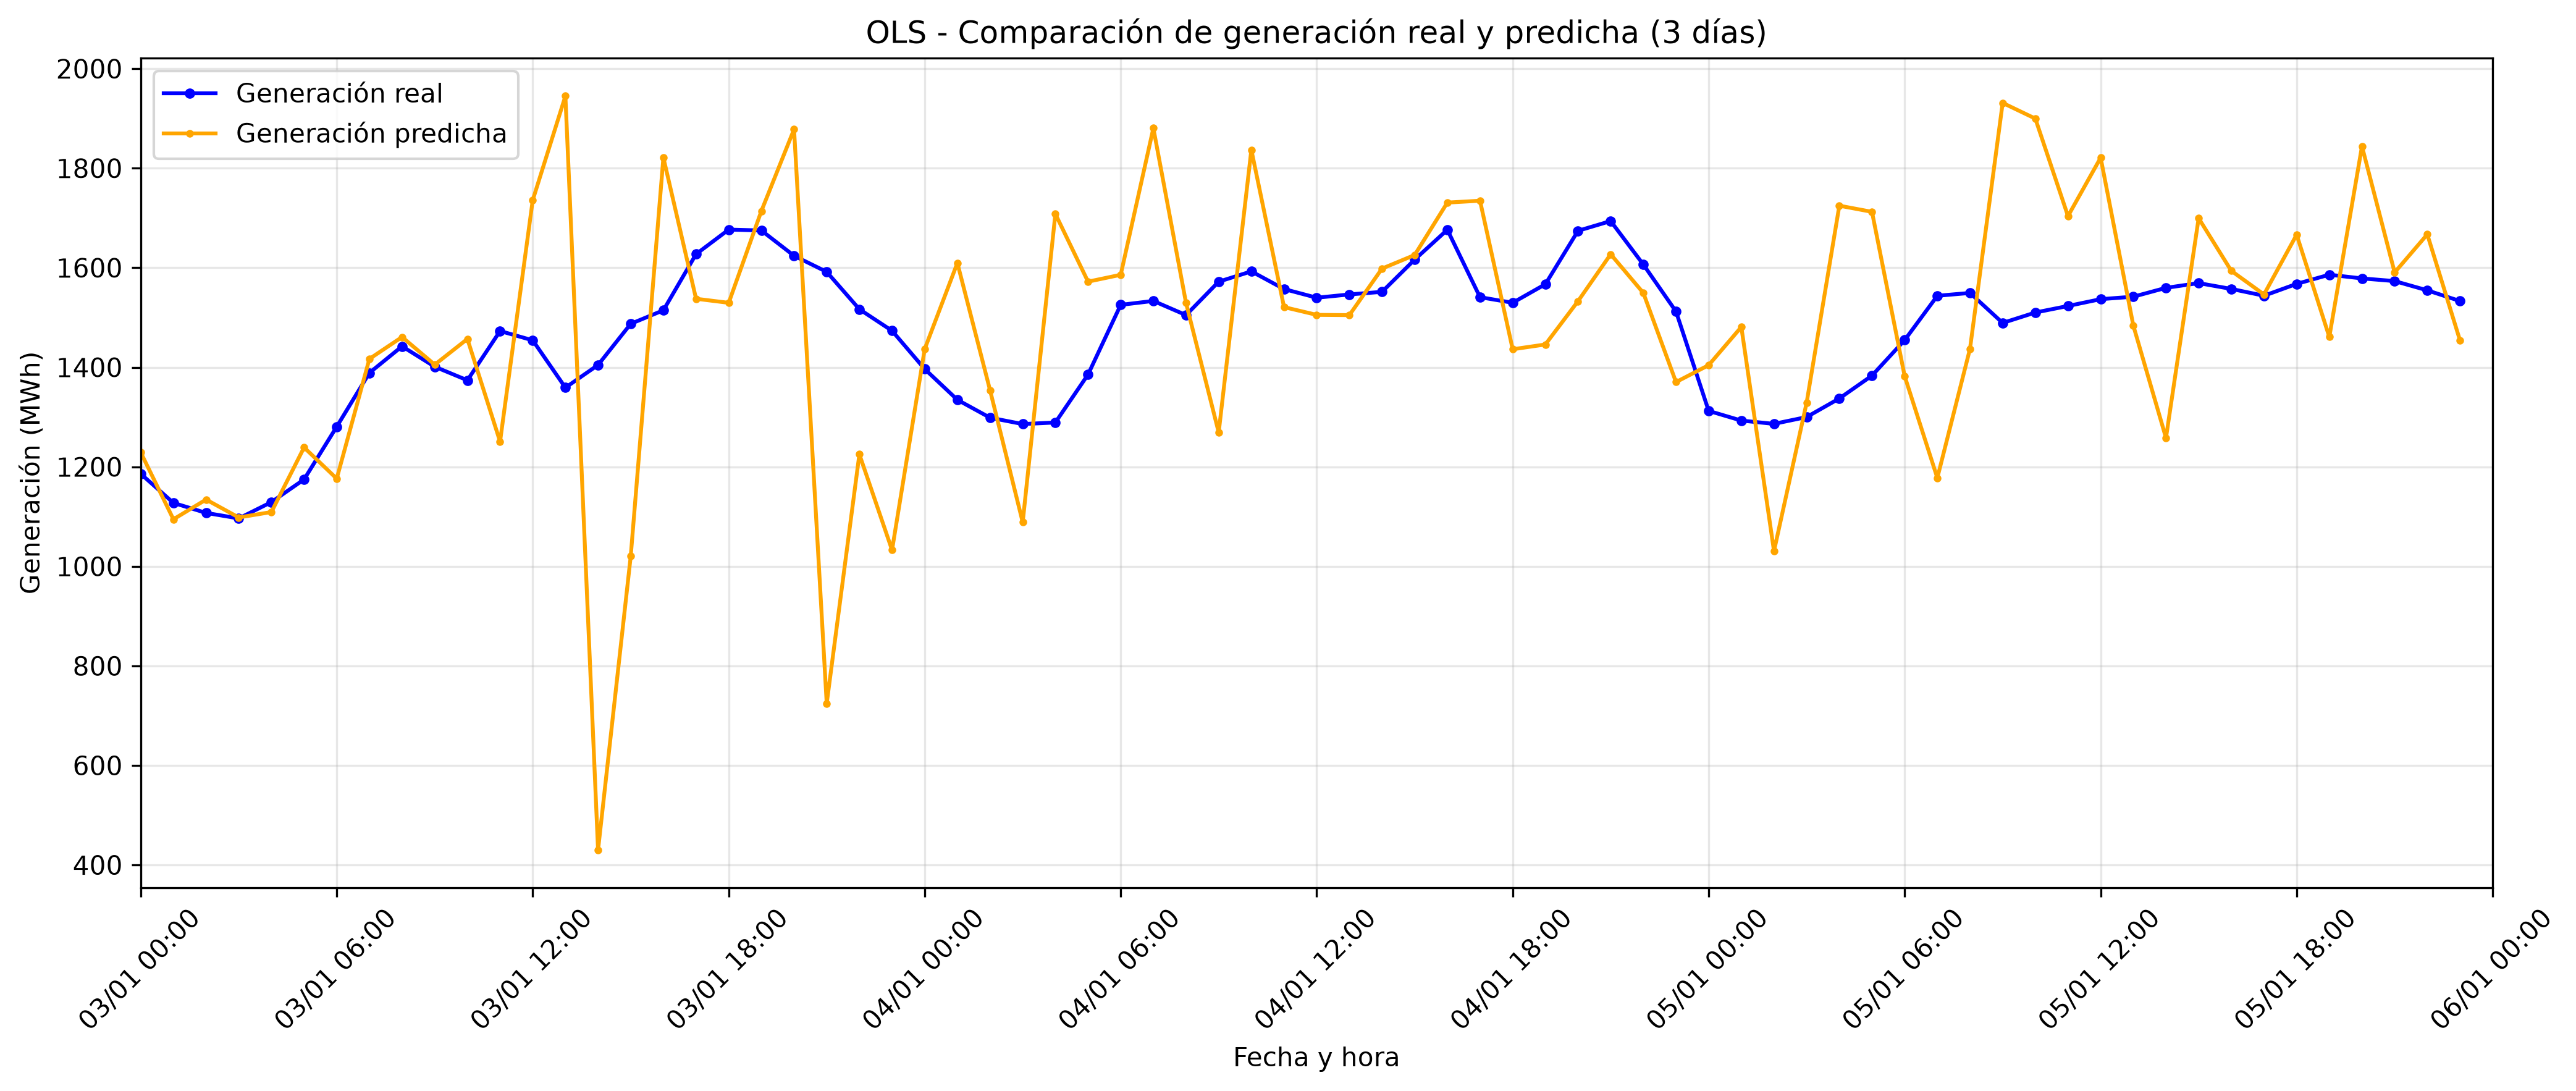
\includegraphics[width=\linewidth]{figuras/prediccion_vs_real_ols_3dias.png}
\caption{OLS. Generación observada y pronosticada durante los primeros tres días desde el inicio de la evaluación individual. Fuente: salida de \texttt{OLS.py}.}
\label{fig:root-ols}
\end{figure}
\FloatBarrier

\paragraph{Ridge, Lasso y Elastic Net con un rezago y calendario.}
Las tres implementaciones usan la generación del registro anterior y cinco variables de calendario\,: hora del día, día del año, año, mes y día de la semana. Cada ventana de 13 filas usa las primeras 12 para ajustar y la última para pronosticar. La selección de $\alpha$ se realiza por validación cruzada de tres particiones dentro de cada ventana con candidatos $0.001$, $0.01$, $0.1$, $1$ y $10$. Elastic Net también considera proporciones $L_1$ de $0.1$, $0.5$ y $0.9$. El eje horizontal de estas figuras enumera las predicciones sucesivas y el eje vertical indica la generación en MWh. El rezago corresponde a la fila previa de la serie filtrada. Si hay huecos en los registros, el avance de un índice puede abarcar más de una hora.

\paragraph{Ridge.}
En la figura~\ref{fig:root-ridge} se puede seguir si la predicción conserva el nivel general de generación y cuánto se aparta en picos y valles. La regularización cuadrática reduce la magnitud de los coeficientes, de modo que el efecto estimado de la fila previa y el calendario se mantiene moderado. Alrededor del índice 4\,000 se aprecia el paso a un nivel de generación más alto. La densidad de las curvas en ese tramo facilita ver el cambio de nivel, pero dificulta distinguir el error de cada observación.

\begin{figure}[!htbp]
\centering
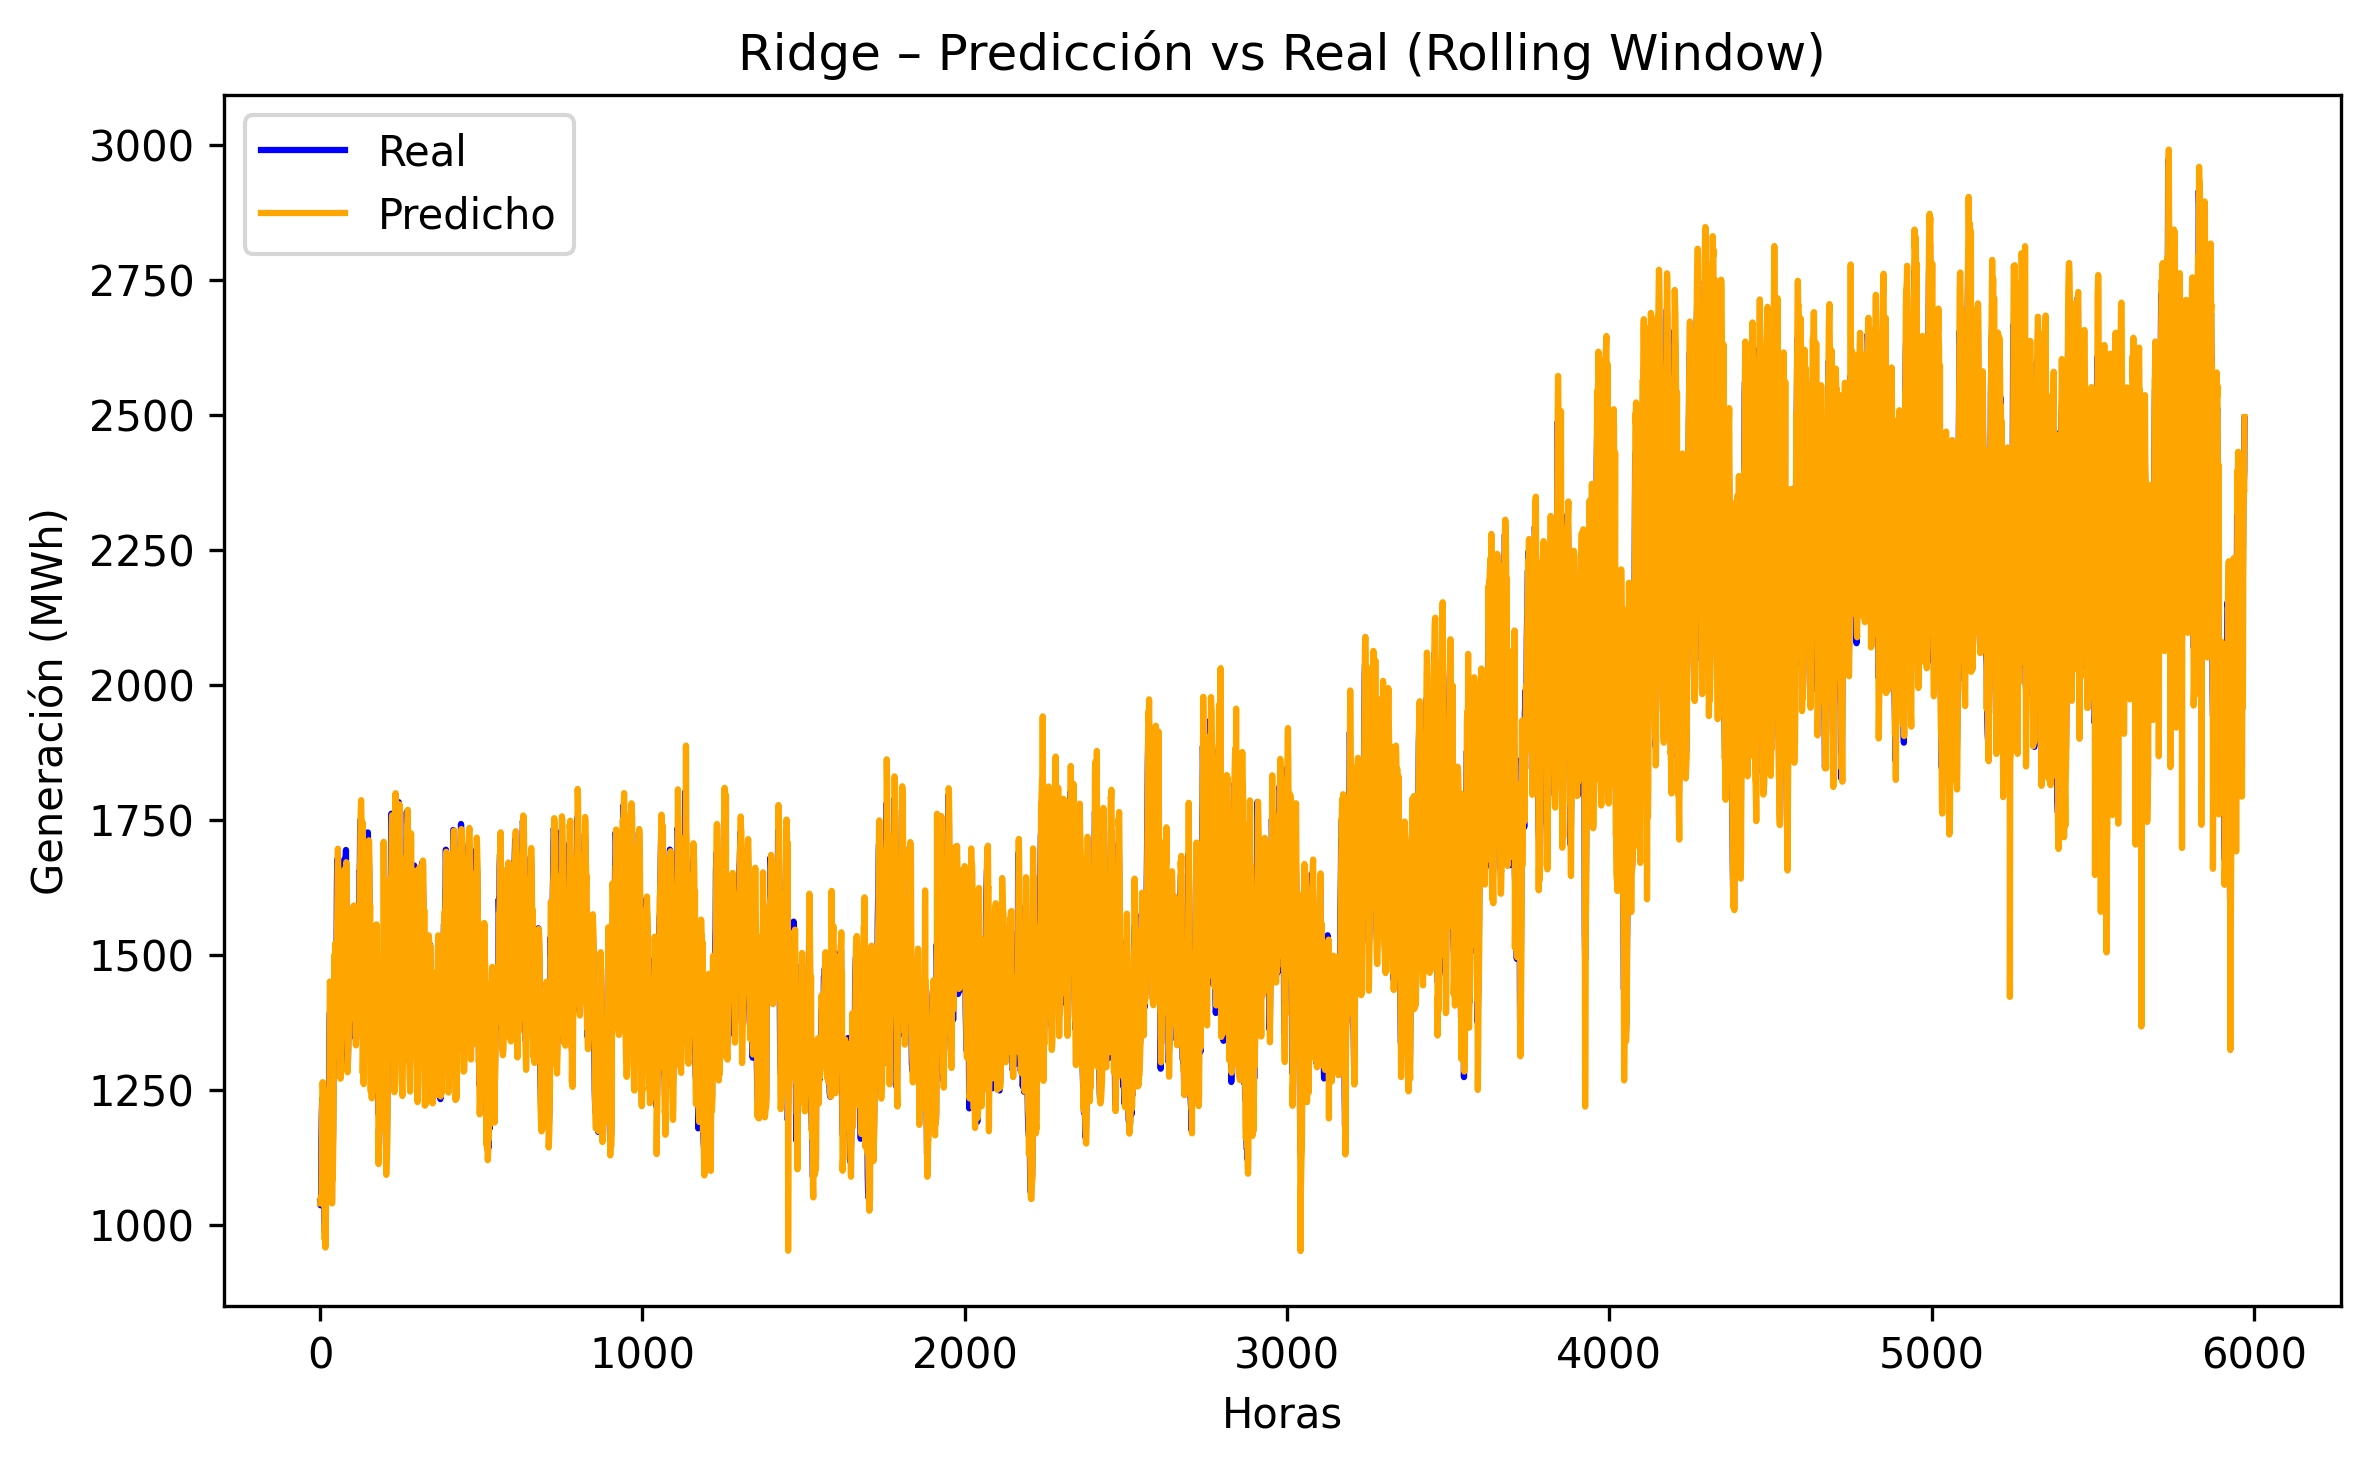
\includegraphics[width=0.88\linewidth]{figuras/prediccion_vs_real_ridge.png}
\caption{Ridge. Generación observada y pronosticada con un rezago y variables de calendario. Fuente: salida de \texttt{ridge.py}.}
\label{fig:root-ridge}
\end{figure}
\FloatBarrier

\paragraph{Lasso.}
La figura~\ref{fig:root-lasso} permite revisar si, después de la penalización absoluta, las predicciones acompañan los ascensos y descensos de la serie. A partir de aproximadamente 4\,000 predicciones, el rango de generación es más amplio y algunos máximos se acercan a 3\,000 MWh. Un acercamiento local facilitaría distinguir qué picos se sobreestiman y cuáles se subestiman. La figura presenta los pronósticos por ventana. Para identificar qué variables tuvieron coeficiente cero haría falta revisar los coeficientes de cada ajuste.

\begin{figure}[!htbp]
\centering
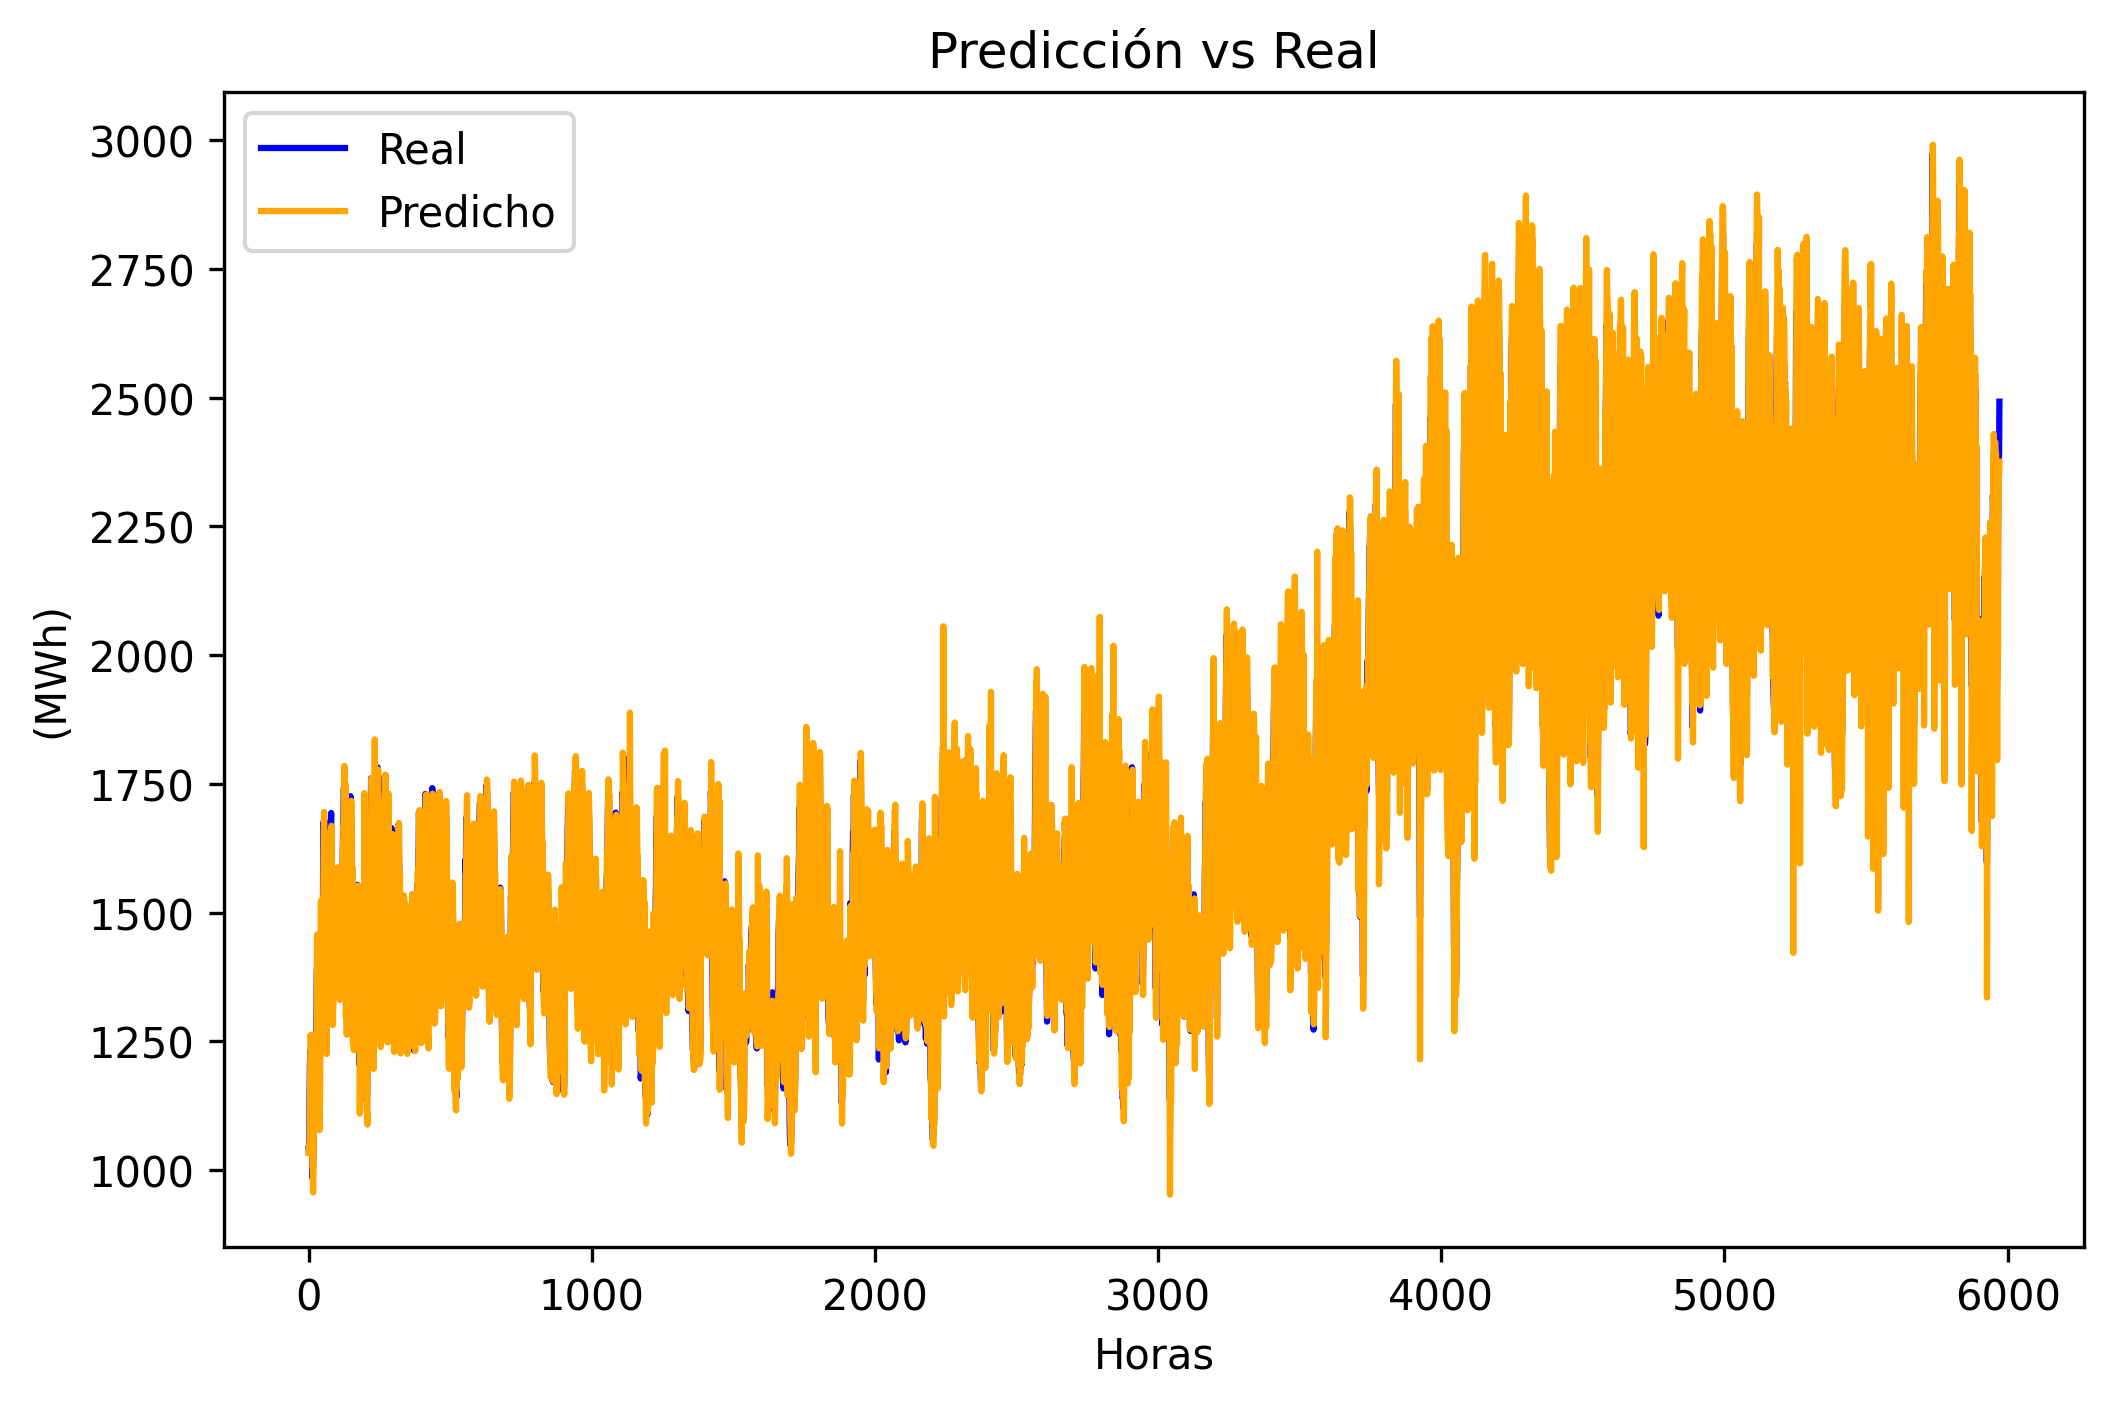
\includegraphics[width=0.88\linewidth]{figuras/prediccion_vs_real_lasso.png}
\caption{Lasso. Generación observada y pronosticada con selección de la penalización en cada ventana. Fuente: salida de \texttt{lasso.py}.}
\label{fig:root-lasso}
\end{figure}
\FloatBarrier

\paragraph{Elastic Net.}
En la figura~\ref{fig:root-elasticnet}, la cercanía entre curvas permite revisar el seguimiento de la generación a lo largo de las ventanas. En la primera parte del gráfico predominan valores entre 1\,000 y 2\,000 MWh. En el tramo final aparecen picos próximos a 3\,000 MWh. La trayectoria pronosticada acompaña ese aumento general del nivel, y la superposición a esta escala dificulta juzgar los errores puntuales. Como cada ajuste selecciona tanto la intensidad total de la penalización como la proporción absoluta, ese equilibrio puede variar durante la evaluación.

\begin{figure}[!htbp]
\centering
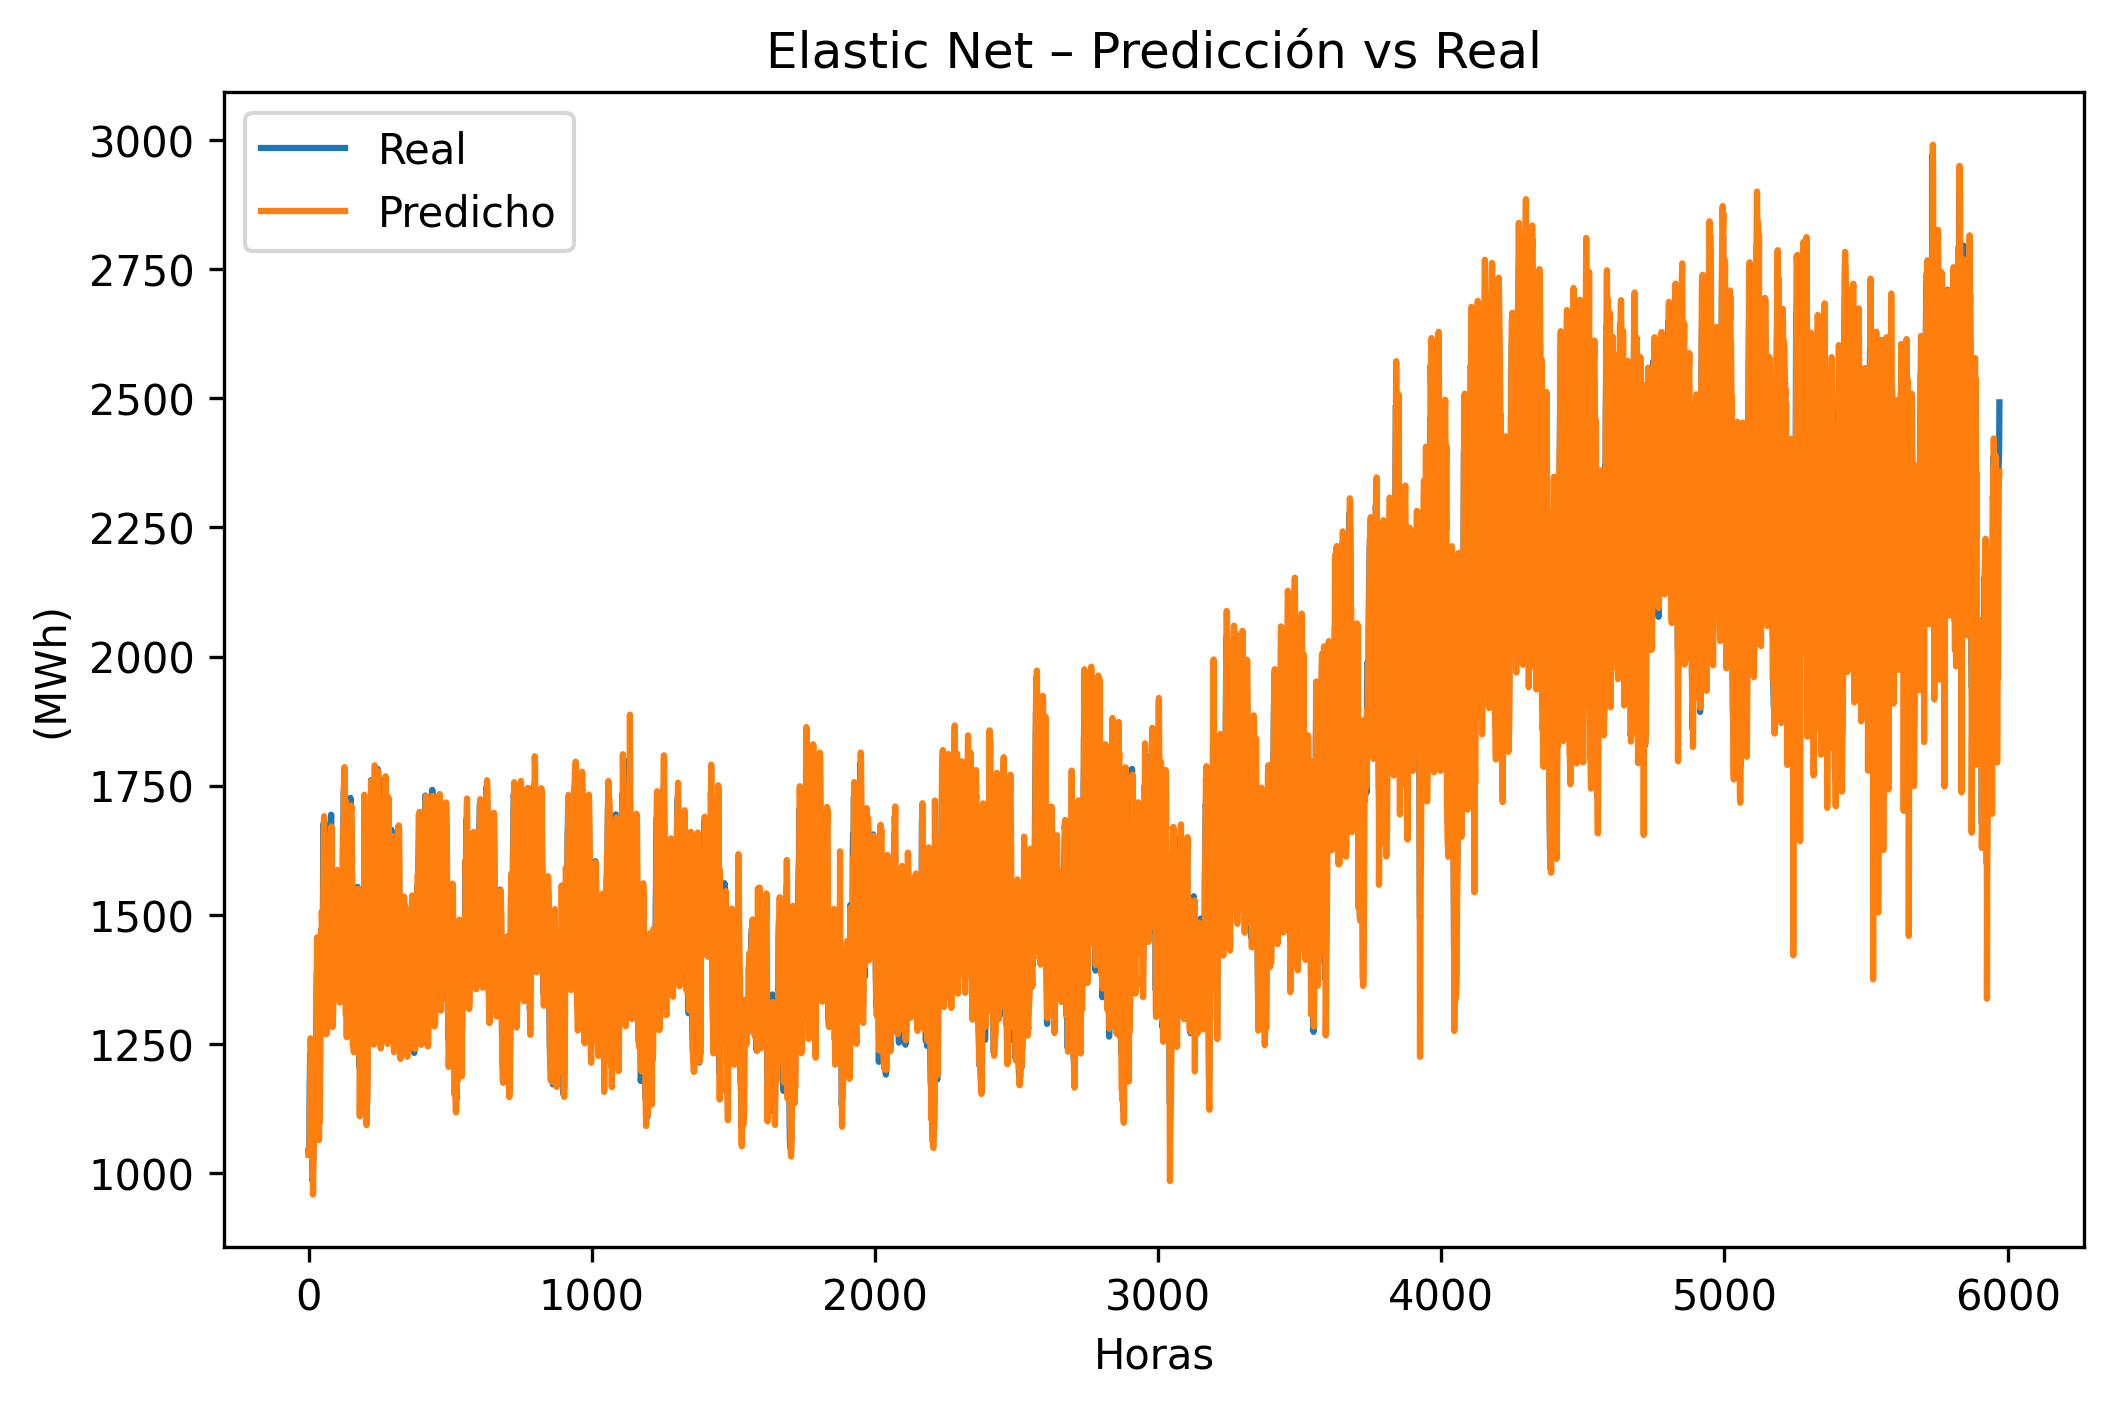
\includegraphics[width=0.88\linewidth]{figuras/prediccion_vs_real_elasticnet.png}
\caption{Elastic Net. Generación observada y pronosticada con penalización mixta ajustada en cada ventana. Fuente: salida de \texttt{Elastic Net.py}.}
\label{fig:root-elasticnet}
\end{figure}
\FloatBarrier
